% !TEX root = Bachelorarbeit_Paul_Zilewitsch.tex

\section{Der Service Desk in GEBman10}

\subsection{Aktuelle Umsetzung}
\noindent
Der Service Desk  ist ein eigenständiges Modul, welches standardmäßig in jeder Version von GEBman10 enthalten ist. Im Dashboard dieses Moduls werden alle Meldungen angezeigt, die erstellt wurden. Rechts daneben wird der Standort des Objektes angezeigt, für das die Meldung aufgegeben wurde. Es werden auch bereits abgeschlossene bzw. erledigte Meldungen angezeigt. Der Benutzer erhält mittels eines Diagramms direkt einen Einblick auf die Meldungen innerhalb einer Woche. Unterteilt wird hierbei in eingegangene Meldungen, Meldungen die in Bearbeitung sind, unbearbeitete Meldungen und fertige Meldungen. Ein zweites Diagramm veranschaulicht die Verweildauer einer Meldung, in dem die Zeit zwischen dem unbearbeiteten Zustand und dem der Bearbeitung protokolliert wird. Unter den beiden Diagrammen finden sich alle Fakten noch einmal in Form von Zahlen wieder. Der Aufbau wird in der Abbildung XX deutlicher. 

\begin{figure}[h!]
\centering
	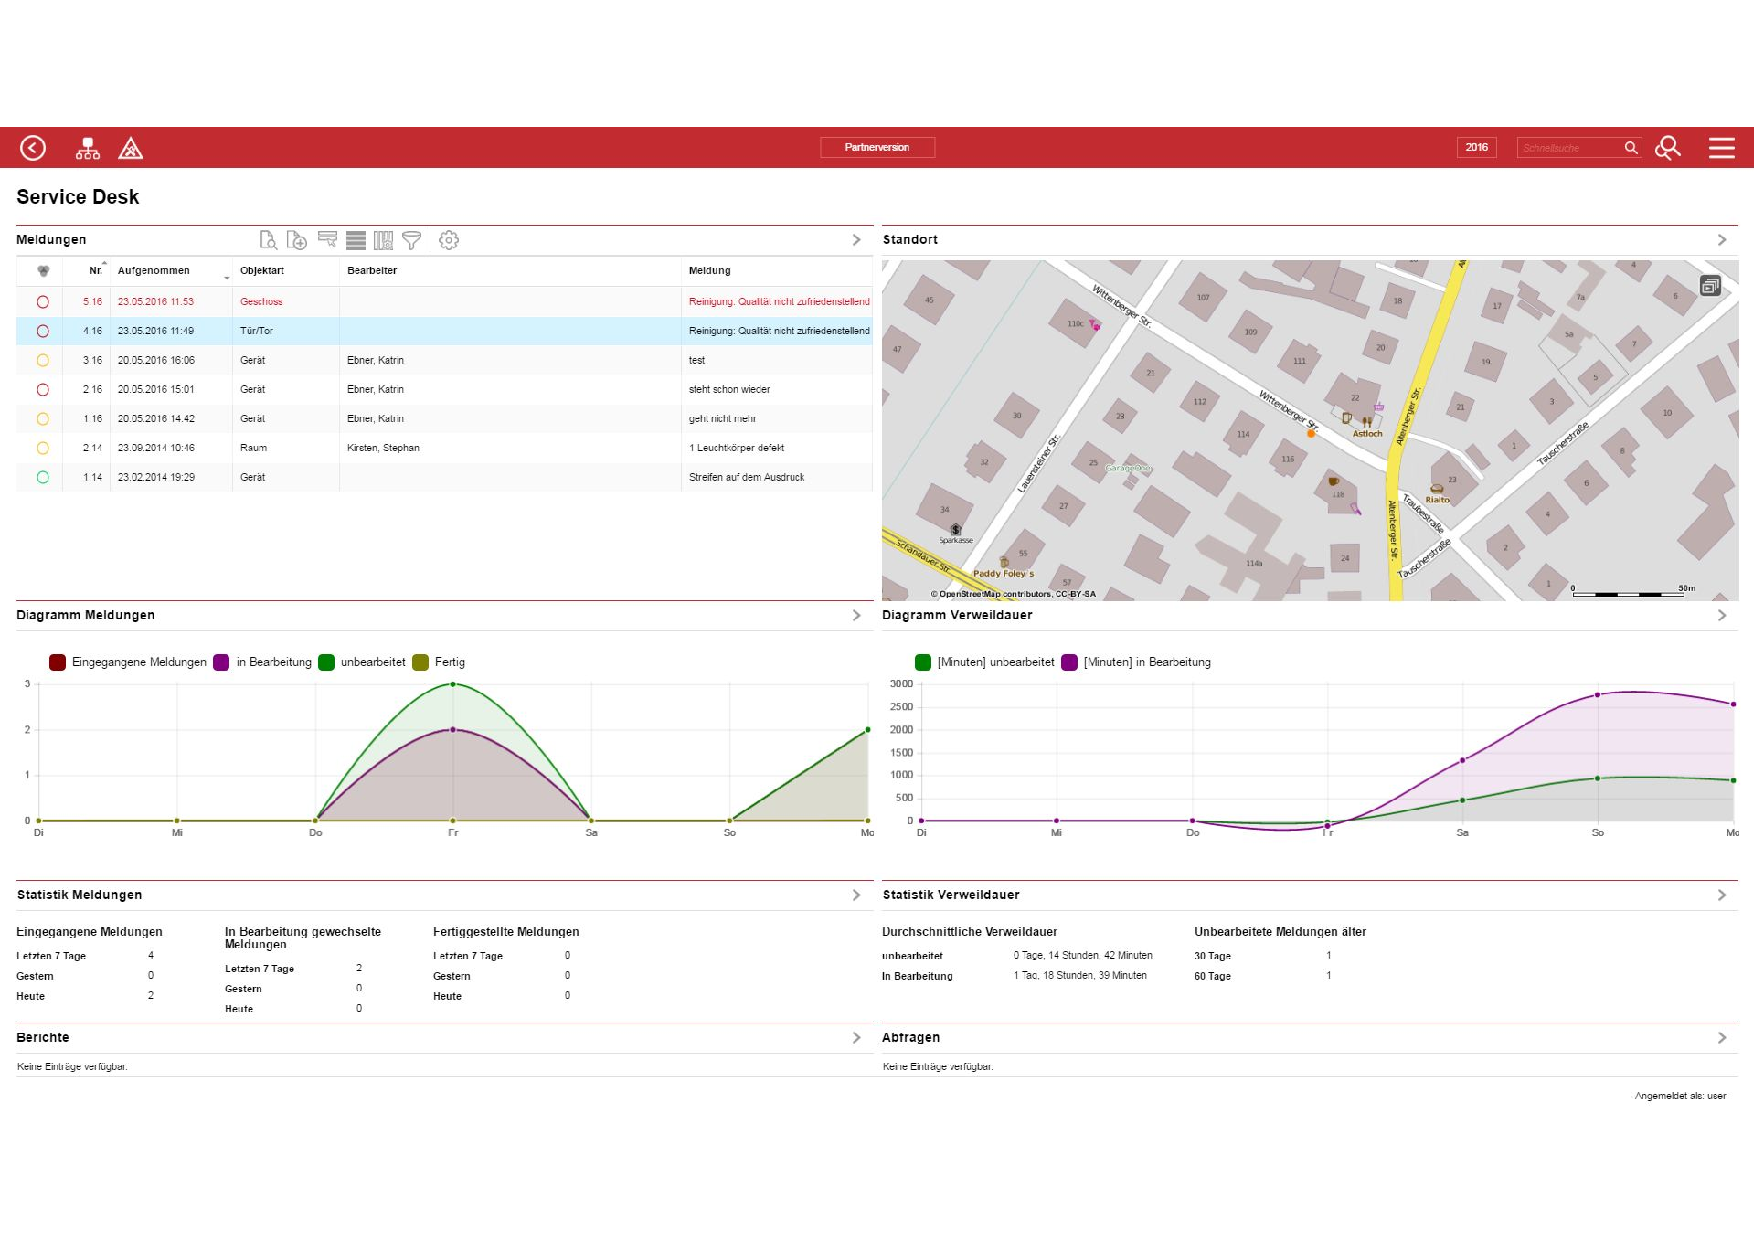
\includegraphics[width=0.75\textwidth]{Abbildungen/GEBman.png}
	\caption[GEBman10 Service Desk Dashboard]{GEBman10 Service Desk Dashboard, Quelle: 
	GEBman10}
	\label{fig:ITIL_Lebenyzyklus}
\end{figure}
\\
\noindent
Der Benutzer hat nun direkt die Möglichkeit für eine Detailansicht einer oder mehrerer Meldung, eine neue Meldung anzulegen, eine Filterung der Meldung vorzunehmen oder die Einstellungen anzupassen.

\subsection{Anforderungen der Erweiterung}

\noindent
Qualität ist ein Maß für das Erfüllen von Anforderungen. Die Qualität des Service Desk kann deshalb nur gesichert werden, wenn die Anforderungen möglichst genau definiert werden. Zu den zu erfüllen Anforderungen sollte aber noch festgehalten werden, welche Anforderungen nicht erfüllt werden sollen. Letzteres wird häufig nicht beachtet, ist jedoch ein wesentlicher Schritt für das Sicherstellen der Anforderungen. \footnote{Vorlesungsreihe Qualitätsmanagement: Hans-Jörg Günther, 6.Semester}\\

\noindent
Aus Kundensicht bestehen leider keine Anforderungen an die E-Mail Integration. Es wurde vor längerer Zeit lediglich mal von einem Kunden gefragt, ob das in Planung ist. Deshalb kann nur auf die Anforderungen Bezug genommen werden, die die KMS Computer GmbH vorgibt und die sich zwangsläufig aus den vorherigen Erkenntnissen ergeben.\\

\noindent
Ziel der Erweiterung des Service Desks ist es, über den E-Mail Kommunikationsweg Meldung zu erstellen, oder auf eingegangene Meldungen zu antworten. Sollten die E-Mail einen Anhang erhalten, muss dieser auch in GEBman 10 abgespeichert werden.\newline
Es soll nicht möglich sein, über die E-Mail Maßnahmen zu generieren, bestehende Meldungen zu löschen oder zu bearbeiten. 


\colorbox{red}{hier muss noch einmal auf alle Punkte von 2. eingegangen werden, um abzugrenzen, was eine Anforderung ist und was eben nicht! }
